
\section{Hall effect}

The Hall effect is a consequence of the Lorentz force on a moving charge. To first understand this we look to the Boltzmann transport equation which allows us to use a semi-classical approach to incorporate the effects of magnetic field to find expressions for single electron transport and in particular the conductivity tensor $\rho$. The Boltzmann transport equation is expressed as follows,
\begin{equation}
    \label{Eqn:Theo:BTE}
     \frac{\partial f}{\partial t} + \vect{v}.\nabla_r f + \vect{F} . \nabla_k f = \left.\frac{d f}{d t}\right|_{\textrm{coll}},
\end{equation}
where $f = f(\vect{r}, \vect{k}, t)$ is the occupation distribution for single electrons at position $\vect{r}$, in state $\vect{k}$ at time $t$ and $\vect{v}$ is the electron velocity, $\vect{F}$ is the force on the electron and the term on the right is the rate of change of the occupation due to collisions. The Boltzmann transport equation arises from the notion that, classically, the chance of occupation of a particular state $f$ at $t$ is equivalent to the probability of occupation of a state at $f - df/dt$ at time $t-dt$. The fact that the equation employs classical dynamics with quantum mechanical Bloch waveforms makes this a semi-classical equation.

The collision term on the right is generally complicated and is usually approximated by the `relaxation time approximation',
\begin{equation}
    \left.\frac{d f}{d t}\right|_{\textrm{coll}} = \frac{f - f_0}{\tau},
\end{equation}
where $f_0$ is the equilibrium occupation distribution to which $f$ tends towards exponentially if the system is perturbed. The rate of the exponential convergence is determined by the relaxation time, $\tau$, with the decay rate of the discrepancy being proportional to $e^{-t/\tau}$.

As discussed in section~\ref{Sec:Theo:dHvAOverview}, electrons at the Fermi surface subject to a magnetic field are confined to orbits of a particular area around the Fermi surface due to the Lorentz force. Dealing solely with the simpler case of closed orbits (c.f. open orbits), we make an approximation of a steady state and uniform distribution so the first two terms of equation~\ref{Eqn:Theo:BTE} are zero. We then incorporate the Lorentz force, $\vect{F} = q(\vect{E} + \vect{V}\times\vect{B})$, in the third term. Finally through some manipulations~\cite{French2009} and on assuming that $k_bT \ll E_F$ so the Fermi distribution is a step function, then we can obtain an expression for the conductivity tensor elements, $\sigma_{ij}$, as the Shockley-Chambers tube integral form of the Boltzmann equation,
\begin{equation}
    \sigma_{ij} = \frac{e^2}{4 \pi^3 \hbar^2}\int \partial k_B \int^{2\pi}_{0} \partial \phi \int^{\infty}_{0} \partial \phi^{\prime} v_i(\phi) v_j(\phi - \phi^{\prime})\frac{m^*}{\omega_c}e^{\phi^{\prime}/(\omega_c \tau)}
\end{equation}
where $\phi$ and $\phi^{\prime}$ are angular integration variables around the orbit. From this integral it is possible to determine the conductivity tensor for a variety of Fermi surface geometries, however given the shape of the \ac{BSCO} Fermi surface, we are most interested in the cylindrical Fermi surface which gives the following conductivity tensor, $\rho$ for a magnetic field applied along $z$,
\begin{equation}
    \rho = \left( \begin{array}{ccc}
                \rho_{xx}   & \rho_{xy} & \rho_{xz} \\
                \rho_{yx}   & \rho_{yy} & \rho_{yz} \\
                \rho_{zx}   & \rho_{zy} & \rho_{zz} \end{array} \right) = \left( \begin{array}{ccc}
                                                        1/\sigma_0  & \omega_c \tau / \sigma_0   & 0  \\
                                                        \omega_c \tau / \sigma_0  & 1/\sigma_0  & 0  \\
                                                        0   & 0 & 0  \end{array} \right)
\end{equation}
where $\omega_c$ is the cyclotron frequency and $\sigma_0$ is the Drude conductivity given by,
\begin{equation}
    \sigma_0 = \frac{ne^2\tau}{m^*}
\end{equation}
where $n$ is the carrier density and $m^*$ is the effective mass. The off-diagonal resistivity component represents the resistivity perpendicular to the current and in the case of $\rho_{xy} (=\rho_{yx})$ is also perpendicular to the field then this is known as the Hall resistivity,
 \begin{equation}
     \rho_{xy} = \frac{\omega_c \tau}{\sigma_0} = \left(\frac{eB}{m^*}\right)\tau\frac{m^*}{ne^2\tau} = \frac{B}{ne}
 \end{equation}
The Hall resistivity can be understood if we consider an electron (hole) moving along a rectangular slab subject to a perpendicular magnetic field. The electrons (holes) are deflected to one side of the slab due to the Lorentz force on the charged particle. Eventually the charge density one one side becomes high enough that the Coulomb repulsion force of the density on subsequent charge carriers balances the Lorentz force and an equilibrium voltage between either side of the slab is reached. This voltage is known as the Hall voltage, $V_H$ and is given by,
\begin{equation}
    V_H = -\frac{I\rho_{xy}}{d} = -\frac{IB}{ned}
\end{equation}
where $I$ and $B_{\perp}$ are the current and perpendicular magnetic field and $n$, $e$ and $d$ are the carrier density, charge and slab thickness respectively. $V_H$ is what is measured in our experiment. This is usually further abstracted to the Hall coefficient, $R_H$, which encapsulates the carrier density for a metal as follows,
\begin{equation}
    R_H = \frac{V_H d}{IB} = \frac{1}{ne}
\end{equation}

Provided the magnetic field is small, meaning $\omega_c \tau \ll 1$, then scattering prevents the formation of Landau tubes described in section~\ref{Sec:Theo:dHvAOverview}. This is known as the low field limit. The high field limit leads to effects such as the quantum Hall effect and quantum oscillations.

% \subsection{Temperature dependent effect of band structure}
% 
% Although there is not an explicit temperature dependent term in the Hall relation above, certain band structure features may affect the carrier density as a function of temperature. Perhaps the best known is that of a region of flat, high \ac{DOS}, band structure close to the Fermi energy which can only be accessed by carriers when the thermal energy is high enough. As described in section~\ref{Sec:Intro:PropertiesBSCO}, there is such a feature in the band structure in the overdoped portion of \ac{BSCO} and many other cuprates.

\subsection{Effects of Fermi surface topology}
    \label{Sec:Theo:TopologyEffects}

Ostensibly, a hole-like Fermi surface would be expected to demonstrate positive Hall coefficient and an electron-like Fermi surface a negative, however it is possible to obtain the exact opposite due to the curvature of the Fermi surface~\cite{Narduzzo2008}. 

For a 2D metal in the weak field semiclassical limit, Ong determined that the transverse conductivity, $\sigma_{xy}$ from which $R_H$ is derived can be obtained by integrating the mean free path vector, $\vect{l_k} = \vect{v_k}\tau_k$ over the Fermi surface ($\vect{v_k}$ is the Fermi velocity and $\tau_k$ is the momentum dependent scattering rate). This is illustrated in figure~\ref{Fig:Theo:NegativeCurvatureLSCO} which integrates over a Fermi surface with a long mean free path in the $(\pi, \pi)$ direction and shows how the resulting $\vect{l_k}$ traces two loops in opposite directions giving rise to a larger `negative' loop from the negative curvature even though the overall surface has a positive curvature.
\begin{figure}[htbp]
    \begin{center}
        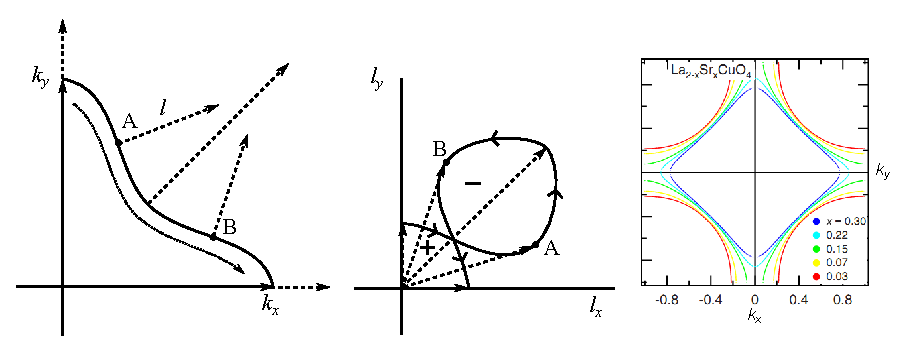
\includegraphics[scale=0.9]{Chapter-Theory/Figures/NegativeCurvatureLSCO/NegativeCurvatureLSCO}
        \caption{Left illustrates a negatively curved Fermi surface with a long mean free path along the $k = (\pi, \pi)$ portion and the integral progressing along the dotted line. Middle shows how the mean free path vector changes along the integral line tracing two loops of opposite direction. Adapted from ref.~\cite{Narduzzo2008}. Right shows the progression of the \ac{BSCO} Fermi surface about the van-Hove singularity. Adapted from ref.~\cite{Kondo2004}.}
        \label{Fig:Theo:NegativeCurvatureLSCO}
    \end{center}
\end{figure}
Narduzzo \etal{} argues that this illustrated scenario is close to what we find in \ac{LSCO} at high doping. Here the mean free path is affected by the anisotropic scattering rate detailed in the introduction section and the proximity of the van-Hove singularity leads to negative curvature in the long flat sides of the Fermi surface as it changes between hole-like and electron-like, as shown for \ac{BSCO} in the right side panel of figure~\ref{Fig:Theo:NegativeCurvatureLSCO}, adapted from ref.~\cite{Kondo2004}.

The form of the equations set out originally by Ong~\cite{Ong1991} for a 2D metal derives a relation for the transverse conductivity, $\sigma_{xy}$ from the Boltzmann model are as follows,
\begin{equation}
    \sigma_{xy} = \frac{e^2}{h}\frac{2\phi}{\phi_0} \hspace{8px}\textrm{where}\hspace{8px}\phi = A_l B
\end{equation}
where $A_l$ is the `Stokes' area traced in the centre panel of figure~\ref{Fig:Theo:NegativeCurvatureLSCO} and $\phi$ is the flux through the Stokes area and $\phi_0 = h/e$ is the flux quantum. The Hall coefficient $R_H$ is given by,
\begin{equation}
    R_HB = \rho_{xy} = \frac{\sigma_{xy}}{\sigma_{xx}\sigma_{yy}}
\end{equation}
where, assuming symmetric scattering along the $x$ and $y$ directions of the conductivity tensor then,
\begin{equation}
    \sigma_{xx} = \sigma_{yy} = \frac{e^2}{4\pi^2 \hbar} \int^{2\pi}_0 k_F(\theta) l(\theta) d\theta
\end{equation} 
Contributions from isotropic scattering which affect $\sigma_{xy}$ are cancelled in $R_H$, however anisotropic scattering at regions of Fermi surface of particular curvature do contribute to the Hall coefficient.
